\documentclass[tikz]{standalone}
\usepackage{fixltx2e}%  http://ctan.org/pkg/fixltx2e

\usepackage[utf8]{inputenx}%  http://ctan.org/pkg/inputenx
% Euler for math | Palatino for rm | Helvetica for ss | Courier for tt
\renewcommand{\rmdefault}{ppl}% rm
\linespread{1.025}% Palatino needs more leading
%\usepackage[scaled]{helvet}% ss //  http://ctan.org/pkg/helvet
%\usepackage{courier}% tt // http://ctan.org/pkg/courier
\usepackage[sc,osf]{mathpazo}
\usepackage[euler-digits,small]{eulervm}  %  http://ctan.org/pkg/eulervm
% a better implementation of the euler package (not in gwTeX)
\normalfont%
\usepackage[T1]{fontenc}%  http://ctan.org/pkg/fontenc
\usepackage{textcomp}%  http://ctan.org/pkg/textcomp
\begin{document}
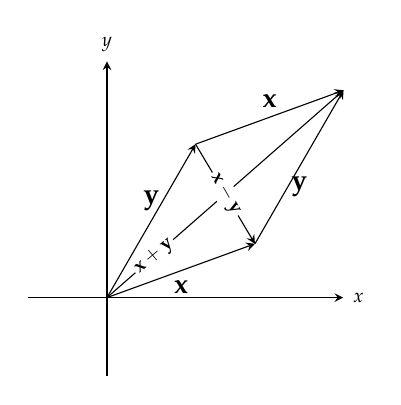
\begin{tikzpicture}
  % draw x and y axis
  \draw[-stealth] (-1cm, 0) -- (3cm, 0) node[right, font = \scriptsize]
  {$x$};
  \draw[-stealth] (0, -1cm) -- (0, 3cm) node[above, font = \scriptsize]
  {$y$};
  % draw x and y vectors
  \def\xang{20}
  \def\yang{60}
  \draw[-stealth] (0, 0) coordinate (O) -- (\xang:2cm) node[pos = 0.5, below]
  {$\mathbf{x}$};
  \draw[-stealth] (O) -- (\yang:2.25cm) node[pos = 0.5, above] {$\mathbf{y}$};
  \draw[-stealth] (\yang:2.25cm) -- ++(\xang:2cm) node[pos = 0.5, above]
  {$\mathbf{x}$};
  \draw[-stealth] (\xang:2cm) -- ++(\yang:2.25cm) coordinate (A)
  node[pos = 0.5, below] {$\mathbf{y}$};
  % draw x + y and x - y
  \draw[-stealth] (O) -- (A) node[rotate = {40}, font = \scriptsize,
  fill = white, inner sep = 0.03cm, pos = 0.2] {$\mathbf{x} + \mathbf{y}$};
  \draw[-stealth] (\yang:2.25cm) -- (\xang:2cm) node[font = \scriptsize,
  inner sep = 0.03cm, fill = white, pos = 0.5, rotate = {-60}]
  {$\mathbf{x} - \mathbf{y}$};
\end{tikzpicture}
\end{document}
%%% Local Variables:
%%% mode: latex
%%% TeX-master: t
%%% End:
